%! TEX program = xelatex

\documentclass[../Postbot.tex]{subfiles}


\begin{document}

	\begin{frame}
		\frametitle{\href{https://developer.twitter.com/en/products/twitter-api}{推特API(1.1)}}
		\begin{columns}
			\begin{column}{.2\textwidth}
				\centering
				{\normalsize 推文} \\
				\hspace*{\fill} \\
				\hspace*{\fill} \\
				\hspace*{\fill} \\
				\hspace*{\fill} \\
				\hspace*{\fill} \\
				\hspace*{\fill} \\
				\hspace*{\fill} \\
				{\normalsize 用户} \\
				\hspace*{\fill} \\
				\hspace*{\fill} \\
			\end{column}

			\begin{column}{.7\textwidth}
				\begin{itemize}
					\item 管理账户设置和信息
					\item 禁言、屏蔽、举报其他用户
					\item 跟随,搜索其他用户
					\item 生成和管理用户列表
					\item 用户信息图片和主页背景
				\end{itemize}
				\hspace*{\fill} \\
				\begin{itemize}
					\item 发布、接受、使用推文
					\item 推特时间轴
					\item 整理推文集
					\item 搜索推文:七天内的
					\item 按照需求过滤实时推文
					\item 样例实时推文
				\end{itemize}
			\end{column}
			
		\end{columns}
	\end{frame}

	\begin{frame}
		\frametitle{\href{https://developer.twitter.com/en/products/twitter-api}{推特API(1.1)}}
		\begin{columns}
			\begin{column}{.2\textwidth}
				\centering
				{\normalsize 直接消息} \\
				\hspace*{\fill} \\
				\hspace*{\fill} \\
				\hspace*{\fill} \\
				\hspace*{\fill} \\
				\hspace*{\fill} \\
				\hspace*{\fill} \\
				\hspace*{\fill} \\
				\hspace*{\fill} \\
				\hspace*{\fill} \\
				{\normalsize 媒体、热点和地理} \\
				\hspace*{\fill} \\
				\hspace*{\fill} \\
			\end{column}

			\begin{column}{.7\textwidth}
				\begin{itemize}{
					\small
					\item 发送和接受事件
					\item 开场消息
					\item 消息附件
					\item 快速回复
					\item 按键
					\item 键入提示符和读取回执
					\item 对话管理
					\item 自定义对话资料
					\item 顾客反馈卡
					}
				\end{itemize}
				\vspace*{\fill} 
				\begin{itemize}{
					\small
					\item 上传媒体文件
					\item 获取接近于某个地区的热点
					\item 获取按照地区整理的热点
					\item 获取关于某个地点的信息
					\item 获取接近于某个地区的地点
				}
				\end{itemize}
			\end{column}
		\end{columns}
	\end{frame}

	\begin{frame}
		\frametitle{\href{https://open.weibo.com/wiki/\%E5\%BE\%AE\%E5\%8D\%9AAPI}{微博API}}
		\begin{columns}
			\begin{column}{.9\textwidth}
				微博 \\ 
				\begin{itemize}
					\item {
						读取接口 \\
						\begin{itemize}
							\item 获取当前登录用户及其所关注用户的最新微博
							\item 获取用户发布的微博
							\item 返回一条原创微博的最新转发微博
							\item 获取@当前用户的最新微博
							\item 根据ID获取单条微博信息
							\item 批量获取指定微博的转发数评论数
							\item 根据ID跳转到单条微博页
							\item 获取官方表情
							\item 第三方分享链接到微博
						\end{itemize}
						}
					\item {
						写入接口 \\
						\begin{enumerate}
							\item 第三方分享链接到微博
						\end{enumerate}
						}
				\end{itemize}
			\end{column}		
		\end{columns}
	\end{frame}

	\begin{frame}
		\frametitle{\href{https://open.weibo.com/wiki/\%E5\%BE\%AE\%E5\%8D\%9AAPI}{微博API}}
		\begin{columns}
			\begin{column}{.9\textwidth}
				评论 \\ 
				\begin{itemize}
					\item {
						读取接口 \\
						\begin{itemize}
							\item 获取某条微博的评论列表
							\item 我发出的评论列表
							\item 我收到的评论列表
							\item 获取用户发送及收到的评论列表
							\item 获取@到我的评论
							\item 批量获取评论内容
						\end{itemize}
						}
					\item {
						写入接口 \\
						\begin{enumerate}
							\item 评论一条微博
							\item 删除一条我的评论
							\item 批量删除我的评论
							\item 回复一条我收到的评论
						\end{enumerate}
						}
				\end{itemize}
			\end{column}		
		\end{columns}
	\end{frame}

	\begin{frame}
		\frametitle{\href{https://open.weibo.com/wiki/\%E5\%BE\%AE\%E5\%8D\%9AAPI}{微博API}}
		\begin{columns}
			\begin{column}{.9\textwidth}
				用户 \\ 
				\begin{itemize}
					\item {
						读取接口 \\
						\begin{enumerate}
							\item 获取用户信息
							\item 通过个性域名获取用户信息
						\end{enumerate}
						}
				\end{itemize}

				公共服务 \\
				\begin{itemize}
					\item {
						读取接口 \\
						\begin{enumerate}
							\item 通过地址编码获取地址名称
							\item 获取城市列表
							\item 获取省份列表
							\item 获取国家列表
							\item 获取时区配置表
						\end{enumerate}
					}
				\end{itemize}
			\end{column}		
		\end{columns}
	\end{frame}

	\begin{frame}
		\frametitle{网页内容接口}
		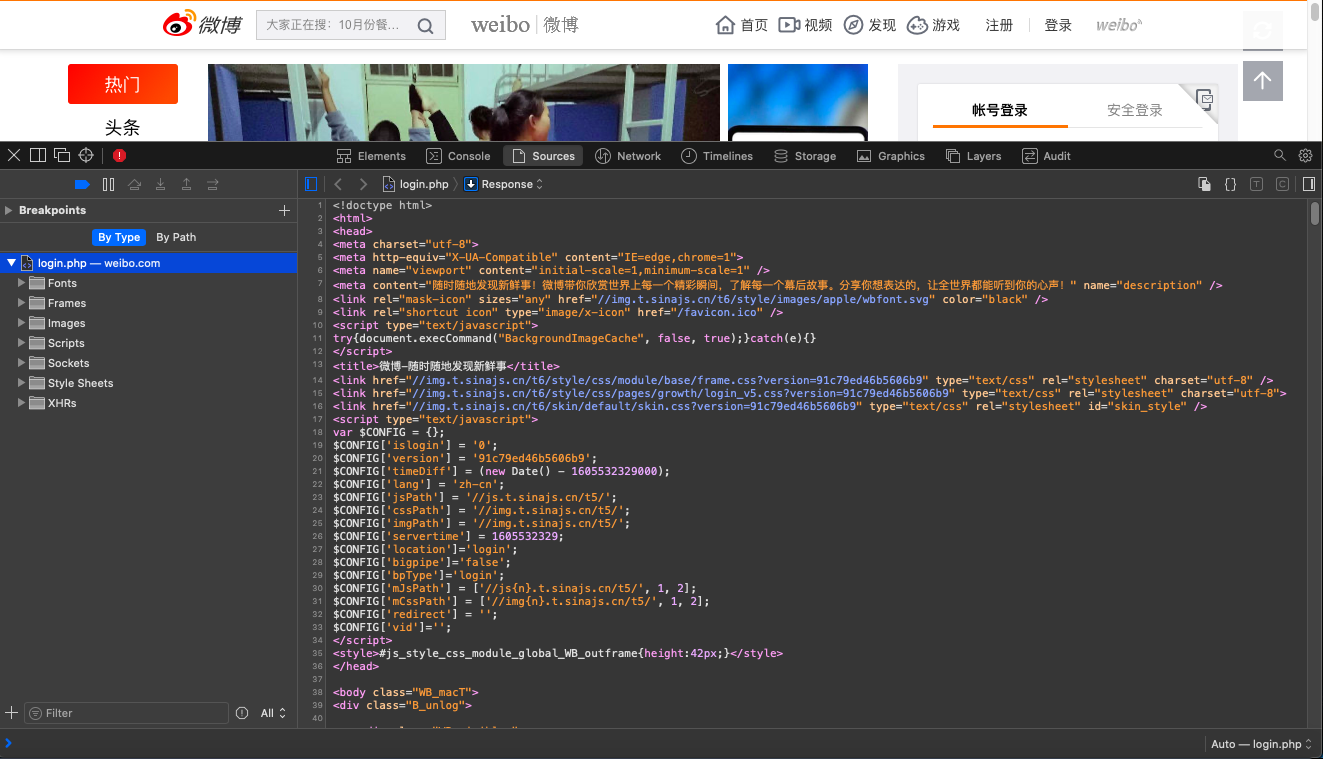
\includegraphics[width=\textwidth]{../src/img/Weibo source code.jpg}
	\end{frame}

\end{document}